\documentclass[12pt]{report}
\usepackage[utf8]{inputenc}
\usepackage[russian]{babel}
%\usepackage[14pt]{extsizes}
\usepackage{listings}
\usepackage{amsmath}
\usepackage[justification=centering]{caption}

\lstdefinelanguage{Kotlin}{
  comment=[l]{//},
  commentstyle={\color{gray}\ttfamily},
  emph={delegate, filter, first, firstOrNull, forEach, lazy, map, mapNotNull, println, return@},
  emphstyle={\color{orange}},
  identifierstyle=\color{black},
  keywords={abstract, actual, as, as?, break, by, class, companion, continue, data, do, dynamic, else, enum, expect, false, final, for, fun, get, if, import, in, interface, internal, is, null, object, override, package, private, public, return, set, super, suspend, this, throw, true, try, typealias, val, var, vararg, when, where, while},
  keywordstyle={\color{blue}\bfseries},
  morecomment=[s]{/*}{*/},
  morestring=[b]",
  morestring=[s]{"""*}{*"""},
  ndkeywords={@Deprecated, @JvmField, @JvmName, @JvmOverloads, @JvmStatic, @JvmSynthetic, Array, Byte, Double, Float, Int, Integer, Iterable, Long, Runnable, Short, String},
  ndkeywordstyle={\color{orange}\bfseries},
  sensitive=true,
  stringstyle={\color{green}\ttfamily},
}

% Для листинга кода:
\lstset{ %
language=Kotlin,                 % выбор языка для подсветки (здесь это С)
basicstyle=\footnotesize\sffamily, % размер и начертание шрифта для подсветки кода
numbers=left,               % где поставить нумерацию строк (слева\справа)
numberstyle=\tiny,           % размер шрифта для номеров строк
stepnumber=1,                   % размер шага между двумя номерами строк
numbersep=5pt,                % как далеко отстоят номера строк от подсвечиваемого кода
showspaces=false,            % показывать или нет пробелы специальными отступами
showstringspaces=false,      % показывать или нет пробелы в строках
showtabs=false,             % показывать или нет табуляцию в строках
frame=single,              % рисовать рамку вокруг кода
tabsize=2,                 % размер табуляции по умолчанию равен 2 пробелам
captionpos=t,              % позиция заголовка вверху [t] или внизу [b] 
breaklines=true,           % автоматически переносить строки (да\нет)
breakatwhitespace=false, % переносить строки только если есть пробел
escapeinside={\#*}{*)}   % если нужно добавить комментарии в коде
}

\usepackage{hyperref}
\hypersetup{
    linktoc=all,     %set to all if you want both sections and subsections linked
    linkcolor=blue,  %choose some color if you want links to stand out
}

% Для измененных титулов глав:
\usepackage{titlesec, blindtext, color} % подключаем нужные пакеты
\definecolor{gray75}{gray}{0.75} % определяем цвет
\newcommand{\hsp}{\hspace{20pt}} % длина линии в 20pt
% titleformat определяет стиль
\titleformat{\chapter}[hang]{\Huge\bfseries}{\thechapter\hsp\textcolor{gray75}{|}\hsp}{0pt}{\Huge\bfseries}

% plot
\usepackage{pgfplots}
\usepackage{filecontents}
\usetikzlibrary{datavisualization}
\usetikzlibrary{datavisualization.formats.functions}

\begin{filecontents}{brut.dat}
3 7768810
4 7224319
5 7990770
6 12360077
7 18466313
8 54640264
9 186935706
10 1332144414
\end{filecontents}

\begin{filecontents}{ant.dat}
3 6373786
4 6397801
5 7014032
6 8505435
7 12679791
8 13791822
9 16966893
10 17774922
\end{filecontents}

\begin{document}
\begin{titlepage}
	\fontsize{12pt}{12pt}\selectfont
	\noindent \begin{minipage}{0.15\textwidth}
		
\includegraphics[width=\linewidth]{inc/img/b_logo.jpg}
	\end{minipage}
	\noindent\begin{minipage}{0.9\textwidth}\centering
		\textbf{Министерство науки и высшего образования Российской Федерации}\\
		\textbf{Федеральное государственное бюджетное образовательное учреждение высшего образования}\\
		\textbf{«Московский государственный технический университет имени Н.Э.~Баумана}\\
		\textbf{(национальный исследовательский университет)»}\\
		\textbf{(МГТУ им. Н.Э.~Баумана)}
	\end{minipage}
	
	\noindent\rule{15cm}{3pt}
	\newline\newline
	\noindent ФАКУЛЬТЕТ \underline{~~~~~~~~~~~~~~~~«Информатика и системы управления»~~~~~~~~~~~~~~~~} \newline\newline
	\noindent КАФЕДРА \underline{«Программное обеспечение ЭВМ и информационные технологии»}\newline\newline\newline\newline\newline\newline\newline
	
	
	\begin{center}
		\Large\textbf{Отчет по лабораторной работе №6 по курсу "Анализ алгоритмов"}\newline
	\end{center}
	
	\noindent\textbf{Тема} \underline{Муравьиный алгоритм}\newline\newline\newline
	\noindent\textbf{Студент} \underline{Якуба Д. В.}\newline\newline
	\noindent\textbf{Группа} \underline{ИУ7-53Б}\newline\newline
	\noindent\textbf{Оценка (баллы)} \underline{~~~~~~~~~~~~~~~~~~~}\newline\newline
	\noindent\textbf{Преподаватели} \underline{Волкова Л.Л., Строганов Ю.В.}\newline
	
	\begin{center}
		\vfill
		Москва~---~\the\year
		~г.
	\end{center}
\end{titlepage}

\setcounter{page}{2}

\tableofcontents

\newpage
\chapter*{Введение}
\addcontentsline{toc}{chapter}{Введение}
\section*{Цель лабораторной работы}
Реализация муравьиного алгоритма и приобретение навыков параметризации методов на примере реализованного алгоритма, примененного к задаче коммивояжера.
\section*{Задачи лабораторной работы}
\begin{enumerate}
\item[1)] изучить алгоритм полного перебора для решения задачи коммивояжера;
\item[2)] реализовать алгоритм полного перебора для решения задачи коммивояжера;
\item[3)] изучить муравьиный алгоритм для решения задачи коммивояжера;
\item[4)] реализовать муравьиный алгоритм для решения задачи коммивояжера;
\item[5)] провести параметризацию муравьиного алгоритма на двух классах данных;
\item[6)] провести сравнительный анализ скорости работы реализованных алгоритмов;
\item[7)] подготовить отчёт по проведенной работе.
\end{enumerate}

\chapter{Аналитическая часть}
В данном разделе описаны задача коммивояжёра, идея муравьиного алгоритма и алгоритма полного перебора для решения этой задачи.

\section{Задача коммивояжера}
Коммивояжёр (фр. commis voyageur) — бродячий торговец. Задача коммивояжёра — важная задача транспортной логистики, отрасли, занимающейся планированием транспортных перевозок \cite{Commie}. В описываемой задаче рассматривается несколько городов  и матрица попарных расстояний между ними. Требуется найти такой порядок  посещения  городов,  чтобы  суммарное  пройденное  расстояние было минимальным, каждый город посещался ровно один раз и  коммивояжер  вернулся  в  тот  город,  с  которого  начал  свой  маршрут.  Другими  словами,  во  взвешенном  полном  графе  требуется 
найти гамильтонов цикл минимального веса.

\section{Алгоритм полного перебора для решения задачи коммивояжера}
Алгоритм полного перебора для решения задачи коммивояжера предполагает рассмотрение всех возможных путей в графе и выбор наименьшего из них.

Такой подход гарантирует точное решение задачи, однако, так как задача относится к числу трансвычислительных \cite{Trans}, то уже при небольшом числе городов решение за приемлемое время невозможно.

\section{Муравьиный алгоритм для решения задачи коммивояжера}
Муравьиные алгоритмы представляют собой новый перспективный метод решения задач оптимизации, в основе которого лежит моделирование поведения колонии муравьев \cite{Ulianov}. Колония представляет собой систему с очень простыми правилами автономного поведения особей.

Каждый муравей определяет для себя маршрут, который необходимо пройти на основе феромона, который он ощущает, во время прохождения, каждый муравей оставляет феромон на своем пути, чтобы остальные муравьи могли по нему ориентироваться. В результате при прохождении каждым муравьем различного маршрута наибольшее число феромона остается на оптимальном пути. 

Самоорганизация колонии является результатом взаимодействия следующих компонентов:
\begin{itemize}
	\item случайность — муравьи имеют случайную природу движения;
	\item многократность — колония допускает число муравьев, достигающее от нескольких десятков до миллионов особей;
	\item положительная обратная связь — во время движения муравей откладывает феромон, позволяющий другим особям определить для себя оптимальный маршрут;
	\item отрицательная обратная связь — по истечении определенного времени феромон испаряется;
	\item целевая функция.
\end{itemize}

Пусть муравей обладает следующими характеристиками:
\begin{itemize}
	\item зрение — определяет длину ребра;
	\item обоняние — чувствует феромон;
	\item память — запоминает маршрут, который прошел.
\end{itemize}

Введем целевую функцию $\eta_{ij} = 1 / D_{ij}$, где $D_{ij}$ — расстояние из текущего пункта $i$ до заданного пункта $j$.

Посчитаем вероятности перехода в заданную точку по формуле \eqref{possibility}:
\begin{equation}
	\label{possibility}
	P_{kij} = \begin{cases}
		\frac{t_{ij}^a\eta_{ij}^b}{\sum_{q=1}^m t^a_{iq}\eta^b_{iq}}, \textrm{вершина не была посещена ранее муравьем k,} \\
		0, \textrm{иначе}
	\end{cases}
\end{equation}
где $a, b$ -- настраиваемые параметры, $t$ - концентрация феромона, причем $a + b = const$, а при $a = 0$ алгоритм вырождается в жадный.

Когда все муравьи завершили движение происходит обновление феромона по формуле \eqref{pheromone1}:
\begin{equation}
	\label{pheromone1}
	t_{ij}(t+1) = (1-p)t_{ij}(t) + \Delta t_{ij}, \Delta t_{ij} = \sum_{k=1}^N t^k_{ij}
\end{equation}
где
\begin{equation}
	\label{pheromone2}
	\Delta t^k_{ij} = \begin{cases}
		Q/L_{k}, \textrm{ребро посещено k-ым муравьем,} \\
		0, \textrm{иначе}
	\end{cases}
\end{equation}
$L_{k}$ — длина пути k-ого муравья, $Q$ — настраивает концентрацию нанесения/испарения феромона, $N$ — количество муравьев.

\section*{Вывод}
Были рассмотрены задача коммивояжера, муравьиный алгоритм и алгоритм полного перебора для решения поставленной задачи.

В данной работе стоит задача реализации двух рассмотренных алгоритмов.

\chapter{Конструкторская часть}
В данном разделе представлены схемы муравьиного алгоритма и алгоритма полного перебора для решения задачи коммивояжера.
\section{Схема алгоритма полного перебора}
Схема алгоритма полного перебора для решения задачи коммивояжера предоставлена на рисунке \ref{img:bruteForce}. Схема алгоритма нахождения всех перестановок в графе, использующаяся в алгоритме полного перебора, предоставлена на рисунке \ref{img:bruteForce2}.

\begin{figure}
\begin{center}
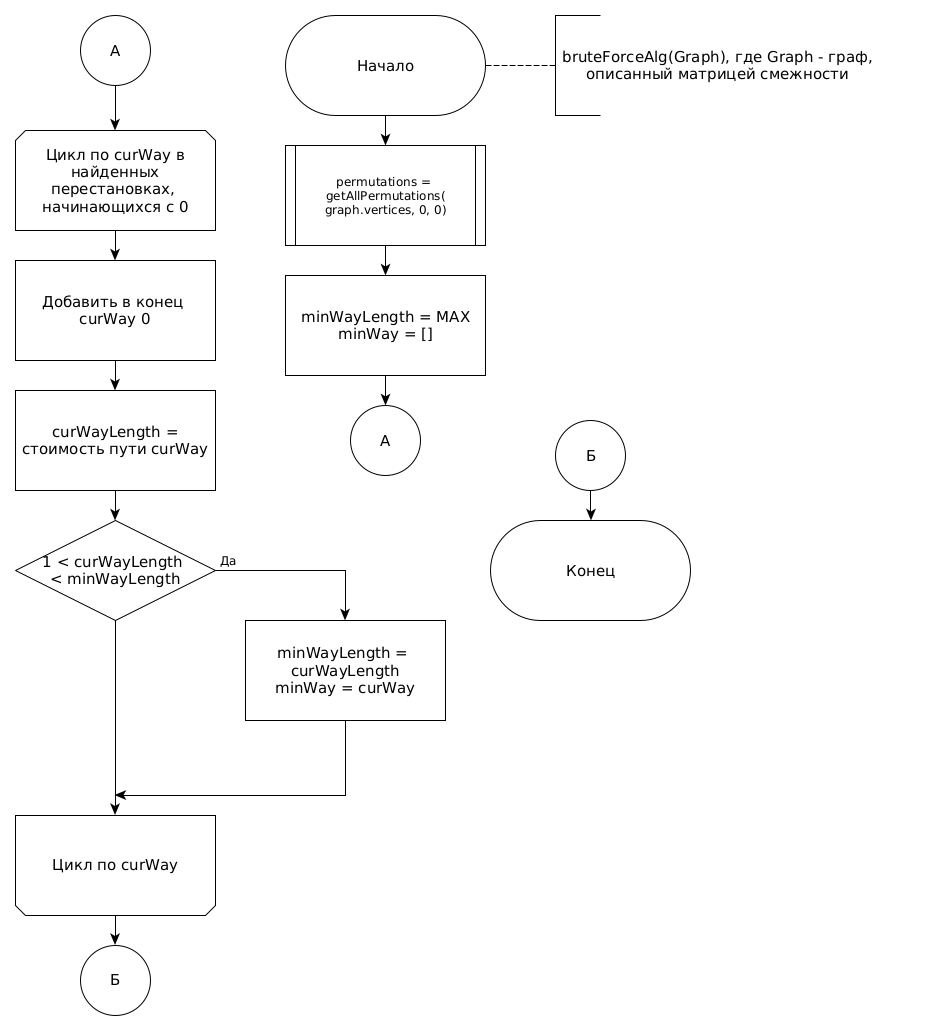
\includegraphics[scale=0.4]{inc/img/bruteForce.png}
\captionsetup{justification=centering}
	\caption{Схема алгоритма полного перебора.}
	\label{img:bruteForce}	
\end{center}
\end{figure}

\begin{figure}
\begin{center}
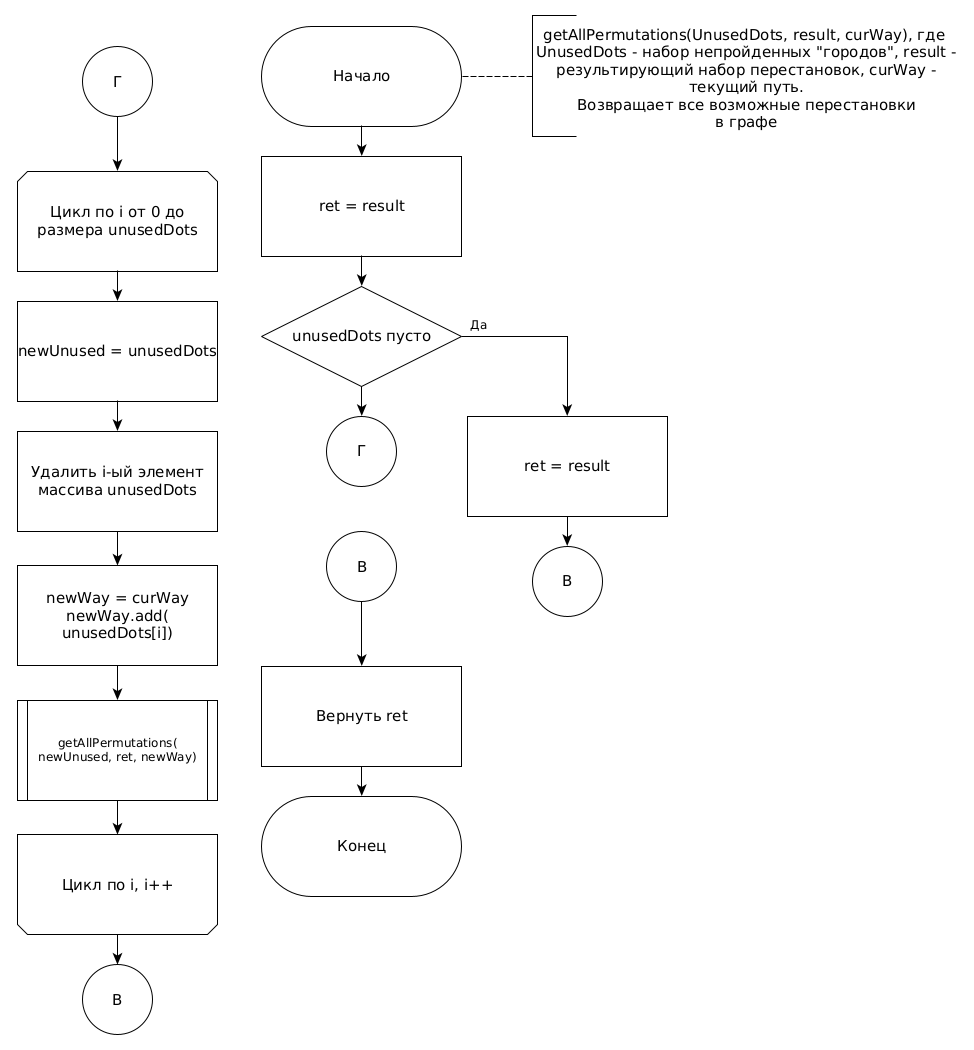
\includegraphics[scale=0.4]{inc/img/bruteForce2.png}
\captionsetup{justification=centering}
	\caption{Схема алгоритма нахождения всех перестановок в графе.}
	\label{img:bruteForce2}	
\end{center}
\end{figure}


\section{Схема муравьиного алгоритма}
На рисункe \ref{img:antAlg} предоставлена схема реализации муравьиного алгоритма для решения задачи коммивояжера.

\begin{figure}[ht]
\begin{center}
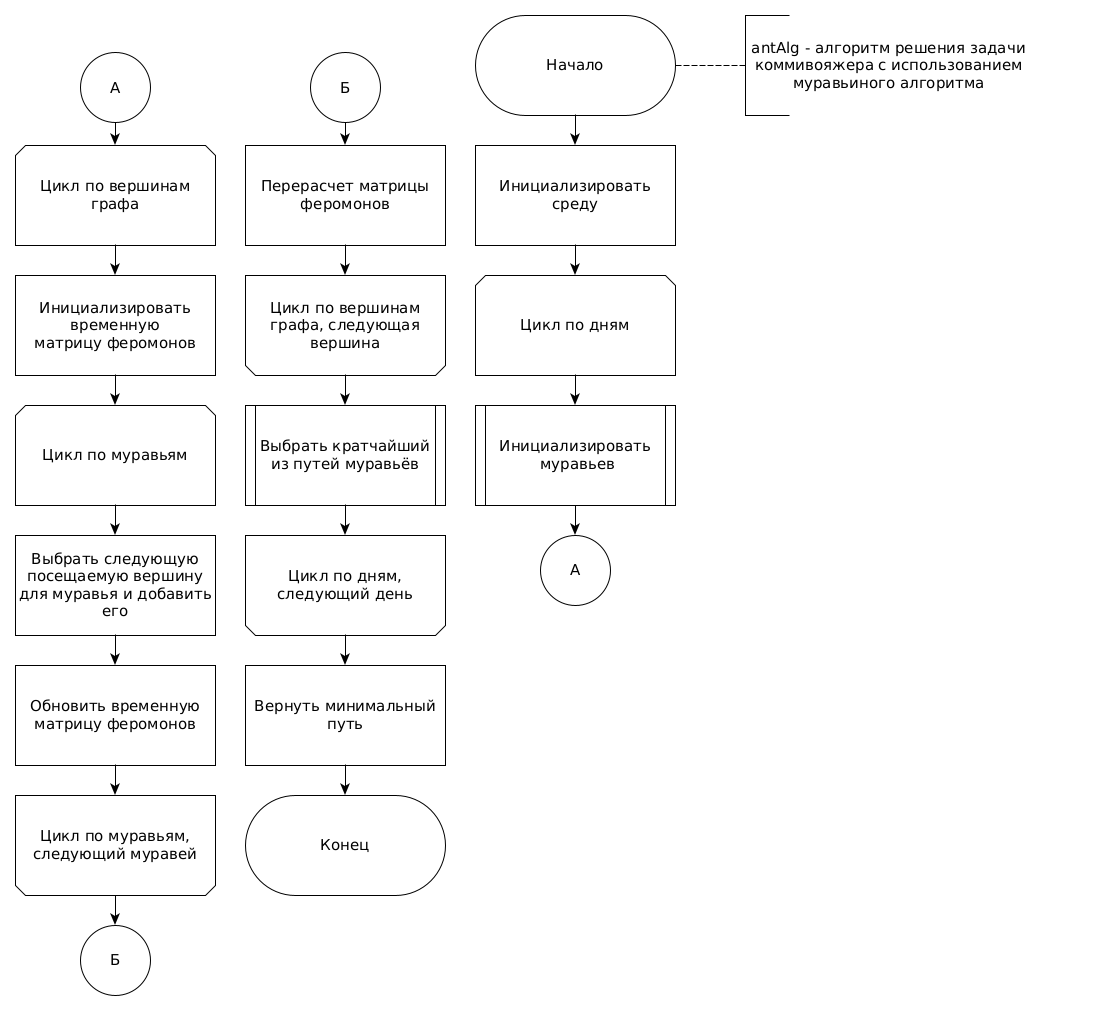
\includegraphics[scale=0.4]{inc/img/antAlg.png}
\captionsetup{justification=centering}
	\caption{Схема реализации муравьиного алгоритма.}
	\label{img:antAlg}	
\end{center}
\end{figure}

\section*{Вывод}
Были представлены схемы алгоритма полного перебора, а муравьиного алгоритма для решения задачи коммивояжера.

\chapter{Технологическая часть}
В данном разделе приведены требования к программному обеспечению, средства реализации программного обеспечения, а также листинг кода.

\section{Требования к программному обеспечению}
\begin{itemize}
\item входные данные - матрица смежности для сильно-связного графа;
\item выходные данные - оптимальные пути, найденные с помощью алгоритма полного перебора и муравьиного алгоритма.
\end{itemize}

\section{Средства реализации программного обеспечения}
При написании программного продукта был задействован язык программирования Kotlin \cite{Kotlin}.

Данный выбор обусловлен следующими факторами:
\begin{itemize}
\item Возможность портирования алгоритмов для работы с Android;
\item Большое количество справочной литературы, связанной с ЯП Java.
\end{itemize}

Для тестирования производительности реализаций алгоритмов использовалась утилита measureTimedValue.

При написании программного продукта использовалась среда разработки IntelliJ IDEA \cite{IntelliJ}.

Данный выбор обусловлен тем, что язык программирования Kotlin - это разработка компании JetBrains, поставляющей данную среду разработки.

\section{Листинг кода}
В листингах \ref{list:Graph} и \ref{list:Colony} предоставлены классы реализации рассматриваемых алгоритмов.
\begin{lstlisting}[caption=Реализация класса графа и  класса графа феромонов,
label={list:Graph}]
const val randomStart = 1
const val randomEnd = 10

class Graph(size_ : Int)
{
    private var size = size_
    private var adjacencyMatrix = Array(size) { IntArray(size) }

    fun setWay(from : Int, to : Int, length : Int)
    {
        adjacencyMatrix[from][to] = length
        adjacencyMatrix[to][from] = length
    }

    fun getWay(from : Int, to : Int) : Int
    {
        return adjacencyMatrix[from][to]
    }

    fun getWayLength(way : MutableList<Int>) : Int
    {
        var length = 0
        for (i in 0 until way.size - 1)
        {
            val curLength = getWay(way[i], way[i + 1])
            length += curLength
        }
        return length
    }

    fun getSize() : Int
    {
        return size
    }

    fun generate()
    {
        for (i in 0 until size)
            for (j in 0 until i)
                setWay(i, j, Random.nextInt(randomStart, randomEnd))
    }

    fun getVertecies() : MutableList<Int>
    {
        val ret : MutableList<Int> = mutableListOf()
        for (i in 0 until size)
            ret.add(i)
        return ret
    }

    fun print()
    {
        for (i in 0 until size)
        {
            for (j in 0 until size)
                print("%3d ".format(getWay(i, j)))
            print('\n')
        }
    }
}

class PheromoneGraph(size_ : Int)
{
    private var size = size_
    private var adjacencyMatrix = Array(size) { DoubleArray(size) }

    fun set(i : Int, j : Int, value : Double)
    {
        adjacencyMatrix[i][j] = value
    }

    fun get(i : Int, j : Int) : Double
    {
        return adjacencyMatrix[i][j]
    }

    fun getSize() : Int
    {
        return size
    }

    fun print()
    {
        for (i in 0 until size)
        {
            for (j in 0 until size)
                print("%5f ".format(get(i, j)))
            print('\n')
        }
    }
}
\end{lstlisting}

\begin{lstlisting}[caption=Класс реализации алгоритма полного перебора для решения задачи коммивояжера,
label={list:BruteForce}]
class BruteForce
{
    fun bruteForceAlg(graph: Graph)
    {
        val permutations = getAllPermutations(graph.getVertecies())

        var minWayLength = MAX_VALUE
        var minWay: MutableList<Int> = mutableListOf()
        for (curWay in permutations.filter { it[0] == 0 })
        {
            curWay.add(0)
            val curWayLength = graph.getWayLength(curWay)
            if (curWayLength in 1 until minWayLength)
            {
                minWayLength = curWayLength
                minWay = curWay
            }
        }

        println("Min way length is: $minWayLength")
        println("Min way is: $minWay")
    }

    private fun getAllPermutations(unusedDots: MutableList<Int>,
                      result : MutableList<MutableList<Int>>? = null,
                      curWay : MutableList<Int>? = null) : MutableList<MutableList<Int>>
    {
        var ret = result
        if (ret == null)
            ret = mutableListOf()

        if (unusedDots.size == 0)
        {
            ret.add(curWay!!)
            return ret
        }

        for (i in 0 until unusedDots.size)
        {
            val newUnusedDots = unusedDots.toMutableList()
            newUnusedDots.removeAt(i)
            var newWay : MutableList<Int> = mutableListOf()
            if (curWay != null)
                newWay = curWay.toMutableList()
            newWay.add(unusedDots[i])

            getAllPermutations(newUnusedDots, ret, newWay)
        }
        return ret
    }
}
\end{lstlisting}

\begin{lstlisting}[caption=Класс реализации муравьиного алгоритма для решения задачи коммивояжера,
label={list:Colony}]
class Colony(graph_: Graph)
{
    var graph = graph_

    class Ant
    {
        var way : MutableList<Int> = mutableListOf()
        var startVertex : Int = 0
        var visitedVerticies = BooleanArray(0)

        var graph = Graph(0)

        constructor(graph_: Graph, startVertex_ : Int)
        {
            way = mutableListOf(startVertex_)
            visitedVerticies = BooleanArray(graph_.getSize())
            startVertex = startVertex_
            visitedVerticies[startVertex_] = true

            graph = graph_
        }

        fun visitVertex(vertex : Int)
        {
            visitedVerticies[vertex] = true
            way.add(vertex)
        }

        fun getWayLength(): Int
        {
            return graph.getWayLength(way)
        }
    }

    val initValue = 0.1

    fun antsInitialization() : MutableList<Ant>
    {
        val ants = mutableListOf<Ant>()
        for (i in 0 until graph.getSize())
            ants.add(Ant(graph, Random.nextInt(0, graph.getSize())))

        return ants
    }

    fun antAlg(days : Int, alpha : Double, beta : Double, rho : Double, q : Double) : Pair<MutableList<Int>, Int>
    {
        var minWay = Int.MAX_VALUE
        var min = mutableListOf<Int>()
        var pheromoneGraph = PheromoneGraph(graph.getSize())

        for (i in 0 until pheromoneGraph.getSize())
        {
            for (j in 0 until pheromoneGraph.getSize())
                pheromoneGraph.set(i, j, initValue)
        }

        for (day in 0 until days)
        {
            val ants = antsInitialization()

            for (i in 0 until graph.getSize() - 1)
            {
                val tempPheromoneGraph = PheromoneGraph(pheromoneGraph.getSize())

                for (curAntNum in 0 until ants.size)
                {
                    var curAnt = ants[curAntNum]
                    var sumChance = 0.0
                    var curVertex = curAnt.way.last()

                    for (vertId in 0 until graph.getSize())
                    {
                        if (!curAnt.visitedVerticies[vertId])
                            sumChance += pheromoneGraph.get(curVertex, vertId).pow(alpha) *
                                    (1.0 / graph.getWay(curVertex, vertId).toDouble()).pow(beta)
                    }

                    var coin = Random.nextDouble()
                    var curChoice = 0
                    while (coin > 0)
                    {
                        if (!curAnt.visitedVerticies[curChoice])
                        {
                            var chance = pheromoneGraph.get(curVertex, curChoice).pow(alpha) *
                                    (1.0 / graph.getWay(curVertex, curChoice).toDouble()).pow(beta) / sumChance
                            coin -= chance
                        }
                        curChoice++
                    }
                    curChoice--

                    ants[curAntNum].visitVertex(curChoice)
                    tempPheromoneGraph.set(curVertex, curChoice,
                            tempPheromoneGraph.get(curVertex, curChoice) +
                                    q / graph.getWay(curVertex, curChoice).toDouble())
                }

                for (k in 0 until graph.getSize())
                    for (j in 0 until graph.getSize())
                        pheromoneGraph.set(k, j, (1 - rho) * pheromoneGraph.get(k, j) + tempPheromoneGraph.get(k, j))
            }

            for (ant in ants)
            {
                ant.way.add(ant.way[0])
                val cur = ant.graph.getWayLength(ant.way)
                if (cur < minWay)
                {
                    minWay = ant.getWayLength()
                    min = ant.way
                }
            }
        }

        return Pair(min, minWay)
    }
}
\end{lstlisting}

\section{Тестирование программного продукта}
В таблице~\ref{tabular:test_rec} приведены тесты для функции, реализующей алгоритм для решения задачи коммивояжера. Тесты пройдены успешно.

\begin{table}[h!]
	\begin{center}
	
	\caption{\label{tabular:test_rec} Тестирование функций}
		\begin{tabular}{c@{\hspace{7mm}}c@{\hspace{7mm}}c@{\hspace{7mm}}c@{\hspace{7mm}}}
			\hline
			Матрица смежности & Ожидаемый наименьший путь \\ \hline
			\vspace{4mm}
			$\begin{pmatrix}
			0 &  3 &  4 &  7\\
			3 &  0 &  3 &  7\\
			4 &  3 &  0 &  7\\
			7 &  7 &  7 &  0
			\end{pmatrix}$ &
			20, [0, 1, 2, 3, 0]\\
			\vspace{2mm}
			\vspace{2mm}
			$\begin{pmatrix}
			0 &  7 &  4 &  3\\
			7 &  0 &  4 &  5\\
			4 &  4 &  0 &  5\\
			3 &  5 &  5 &  0
			\end{pmatrix}$ &
			16, [0, 2, 1, 3, 0]\\
			\vspace{2mm}
			\vspace{2mm}
			$\begin{pmatrix}
			0 &  8 &  9 &  7\\
			8 &  0 &  4 &  4\\
			9 &  4 &  0 &  2\\
			7 &  4 &  2 &  0
			\end{pmatrix}$ &
			21, [0, 1, 2, 3, 0]\\
		\end{tabular}
	\end{center}
\end{table}

\section*{Вывод}
Спроектированные алгоритмы были реализованы и протестированы.

\chapter{Исследовательская часть}
\section{Технические характеристики}
Технические характеристики ЭВМ, на котором выполнялись исследования:
\begin{itemize}
\item ОС: Manjaro Linux 20.1.1 Mikah;
\item Оперативная память: 16 Гб;
\item Процессор: Intel Core i7-10510U.
\end{itemize}

При проведении замеров времени ноутбук был подключен к сети электропитания.

\section{Пример работы программного обеспечения}
На рисунке \ref{img:example} приведен пример работы программы.

\begin{figure}
\begin{center}
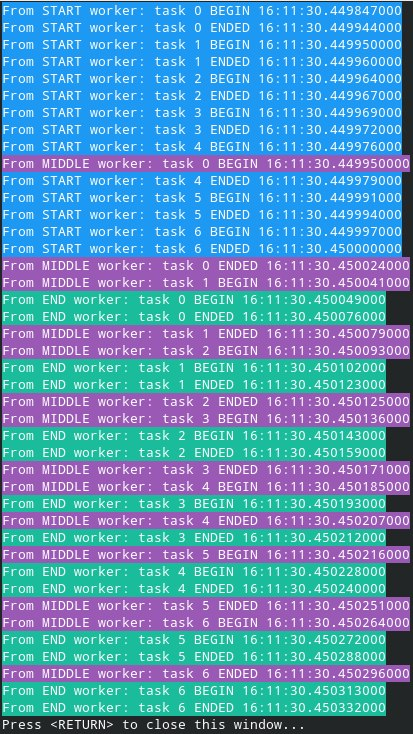
\includegraphics[scale=0.9]{inc/img/example.png}
\captionsetup{justification=centering}
	\caption{Пример работы ПО.}
	\label{img:example}	
\end{center}
\end{figure}
\newpage

\section{Исследование скорости работы алгоритмов}
Алгоритмы тестировались на данных, сгенерированных случайным образом один раз.

Результаты замеров времени приведены в таблице \ref{time1}. На рисунке \ref{timeRes1} приведен графики зависимостей времени работы алгоритмов от размерности матрицы смежности.


\begin{table}[h]
	\begin{center}
		\caption{\label{time1} Замеры времени}
		\begin{tabular}{|c | c | c|} 
 			\hline
			Размерность матрицы & Полный перебор & Муравьиный алгоритм\\ [0.5ex] 
 			\hline\hline
 			3 & 7768810 & 6373786\\
 			\hline
 			4 & 7224319 & 6397801\\
 			\hline
			5 & 7990770 & 7014032\\
			\hline
			6 & 12360077 & 8505435\\
			\hline
			7 & 18466313 & 12679791\\
			\hline
			8 & 54640264 & 13791822\\
			\hline
			9 & 186935706 & 16966893\\
			\hline
			10 & 1332144414 & 17774922\\
			\hline
			\end{tabular}
	\end{center}
\end{table}

\begin{figure}[h]
\begin{center}
	\begin{tikzpicture}
	
\begin{axis}[
  		  	axis lines = left,
  		  	xlabel = размер,
  		  	ylabel = {время, нс},
			legend pos=north west,
			ymajorgrids=true
		] 
		\addplot[color=orange] table[x index=0, y index=1] {brut.dat};
		\addplot[color=blue, mark=square] table[x index=0, y index=1] {ant.dat};

		\addlegendentry{Полный перебор}
		\addlegendentry{Муравьиный алгоритм}
		\end{axis}
	\end{tikzpicture}
	\captionsetup{justification=centering}
	\caption{Зависимость времени работы от размера матрицы смежности}
	\label{timeRes1}
	\end{center}
\end{figure}

\newpage

\section{Постановка эксперимента}
В муравьином алгоритме вычисления производятся на основе настраиваемых параметров.
Рассмотрим два класса данных и подберем к ним параметры, при которых метод даст точный результат при минимальном количестве итераций.

Будем рассматривать матрицы размерности $10\times10$, так как иначе получение точного результата алгоритмом полного перебора слишком велико.

В качестве первого класса данных выделим матрицу смежности, в которой все значения незначительно отличаются друг от друга, например, в диапазоне $[1, 25]$.
Вторым классом будут матрицы, где значения могут значительно отличаться, например $[1, 15000]$.

Будем запускать муравьиный алгоритм для всех значений $\alpha, \rho\in[0, 1]$, с шагом $= 0.1$, пока не будет найдено точное значение для каждого набора.

В результате тестирования будет выведена таблица со значениями $\alpha, \beta, \rho$, $days$, $ dist$, где $days$ — количество дней, данных для решения задачи, $dist$ - определённая алгоритмом длина оптимального пути, а $\alpha, \beta, \rho$ — настроечные параметры.

\subsection{Класс данных 1}
\begin{equation}
\label{matrix}
	M = \begin{pmatrix}
		0 &  3 & 14 &  2 & 22 & 20 &  2 & 14 & 18 & 23\\
		3 &  0 & 12 & 12 &  8 & 24 & 19 &  4 & 20 & 12\\
		14 & 12 & 0 & 23 &  8 &  3 & 21 & 16 &  6 &  5\\
		2 & 12 & 23 &  0 & 22 & 19 &  1 & 13 & 15  & 8\\
		22 &  8 &  8 & 22 &  0 &  8 &  2  & 8 & 11 &  7\\
		20 & 24 &  3 & 19 &  8  & 0 & 15 & 12 & 18  & 9\\
		2 & 19 & 21  & 1 &  2 & 15  & 0 & 13 & 18 & 21\\
		14 &  4 & 16 & 13 &  8 & 12 & 13 &  0 &  7 & 23\\
		18 & 20 &  6 & 15 & 11 & 18 & 18 &  7 &  0 & 19\\
		23 & 12 &  5  & 8 &  7 &  9 & 21 & 23 & 19 &  0
	\end{pmatrix}
\end{equation}

В таблице ~\ref{T:log111} приведены результаты параметризации метода решения задачи коммивояжера на основании муравьиного алгоритма. Полный перебор определил оптимальную длину пути 44.

\begin{table}
	\caption{Таблица коэффициентов для класса данных №1}
	\begin{minipage}[h!]{0.10\hsize}\centering
		\begin{center}\resizebox{4\textwidth}{!}{%
			\begin{tabular}{c@{\hspace{5mm}}c@{\hspace{5mm}}c@{\hspace{5mm}}c@{\hspace{5mm}}c@{\hspace{5mm}}c}
				\toprule
				\alpha        & \beta      & \rho      &days &длина пути \\
				\midrule
				0       &1      &0      &50    &47\\
				0       &1      &0.1    &50    &44\\
				0       &1      &0.2    &50    &49\\
				0       &1      &0.3    &50    &44\\
				0       &1      &0.4    &50    &52\\
				0       &1      &0.5    &50    &51\\
				0       &1      &0.6    &50    &44\\
				0       &1      &0.7    &50    &44\\
				0       &1      &0.8    &50    &44\\
				0       &1      &0.9    &50    &51\\
				0       &1      &1      &50    &44\\
				\midrule
				0.1     &0.9    &0      &50     &44\\
				0.1     &0.9    &0.1    &50    &47\\
				0.1     &0.9    &0.2    &50   &44\\
				0.1     &0.9    &0.3    &50   &44\\
				0.1     &0.9    &0.4    &50    &44\\
				0.1     &0.9    &0.5    &50    &47\\
				0.1     &0.9    &0.6    &50    &44\\
				0.1     &0.9    &0.7    &50   &44\\
				0.1     &0.9    &0.8    &50   &44\\
				0.1     &0.9    &0.9    &50   &44\\
				0.1     &0.9    &1      &50    &67\\
				\midrule
				0.2     &0.8    &0      &50    &44\\
				0.2     &0.8    &0.1    &50    &44\\
				0.2     &0.8    &0.2    &50    &44\\
				0.2     &0.8    &0.3    &50    &44\\
				0.2     &0.8    &0.4    &50    &44\\
				0.2     &0.8    &0.5    &50    &44\\
				0.2     &0.8    &0.6    &50    &44\\
				0.2     &0.8    &0.7    &50    &44\\
				0.2     &0.8    &0.8    &50    &44\\
				0.2     &0.8    &0.9    &50    &44\\
				0.2     &0.8    &1      &50     &93\\
				\midrule
				0.3     &0.7    &0      &50    &44\\
				0.3     &0.7    &0.1    &50    &44\\
				0.3     &0.7    &0.2    &50    &44\\
				0.3     &0.7    &0.3    &50    &44\\
				0.3     &0.7    &0.4    &50    &44\\
				0.3     &0.7    &0.5    &50    &44\\
				0.3     &0.7    &0.6    &50    &49\\
				0.3     &0.7    &0.7    &50    &44\\
				0.3     &0.7    &0.8    &50    &44\\
				0.3     &0.7    &0.9    &50   &52\\
				0.3     &0.7    &1      &50    &88\\
				\bottomrule
			\end{tabular}}
			\label{T:log111}
		\end{center}
	\end{minipage}
	\hfill
	\begin{minipage}[!h]{0.50\hsize}\centering
		\begin{center}\resizebox{0.8\textwidth}{!}{%
			%\caption{Лог работы программы.}
			\begin{tabular}{c@{\hspace{5mm}}c@{\hspace{5mm}}c@{\hspace{5mm}}c@{\hspace{5mm}}c@{\hspace{5mm}}c}
				\toprule
				\alpha        & \beta      & \rho      &days &длина пути \\
				\midrule
				0.4     &0.6    &0      &50    &44\\
				0.4     &0.6    &0.1    &50    &44\\
				0.4     &0.6    &0.2    &50    &44\\
				0.4     &0.6    &0.3    &50    &44\\
				0.4     &0.6    &0.4    &50    &44\\
				0.4     &0.6    &0.5    &50    &44\\
				0.4     &0.6    &0.6    &50    &44\\
				0.4     &0.6    &0.7    &50    &44\\
				0.4     &0.6    &0.8    &50    &44\\
				0.4     &0.6    &0.9    &50    &53\\
				0.4     &0.6    &1      &50     &93\\
				\midrule
				0.5     &0.5    &0      &50    &44\\
				0.5     &0.5    &0.1    &50    &44\\
				0.5     &0.5    &0.2    &50    &44\\
				0.5     &0.5    &0.3    &50    &44\\
				0.5     &0.5    &0.4    &50    &44\\
				0.5     &0.5    &0.5    &50    &47\\
				0.5     &0.5    &0.6    &50    &53\\
				0.5     &0.5    &0.7    &50    &59\\
				0.5     &0.5    &0.8    &50    &44\\
				0.5     &0.5    &0.9    &50   &62\\
				0.5     &0.5    &1      &50    &77\\
				\midrule
				0.6     &0.4    &0      &50    &44\\
				0.6     &0.4    &0.1    &50    &44\\
				0.6     &0.4    &0.2    &50    &44\\
				0.6     &0.4    &0.3    &50    &44\\
				0.6     &0.4    &0.4    &50    &44\\
				0.6     &0.4    &0.5    &50    &49\\
				0.6     &0.4    &0.6    &50    &44\\
				0.6     &0.4    &0.7    &50   &52\\
				0.6     &0.4    &0.8    &50    &58\\
				0.6     &0.4    &0.9    &50    &59\\
				0.6     &0.4    &1      &50    &93\\
				\midrule
				0.7     &0.3    &0      &50    &44\\
				0.7     &0.3    &0.1    &50    &44\\
				0.7     &0.3    &0.2    &50    &49\\
				0.7     &0.3    &0.3    &50    &49\\
				0.7     &0.3    &0.4    &50    &44\\
				0.7     &0.3    &0.5    &50    &47\\
				0.7     &0.3    &0.6    &50    &52\\
				0.7     &0.3    &0.7    &50    &57\\
				0.7     &0.3    &0.8    &50    &51\\
				0.7     &0.3    &0.9    &50    &54\\
				0.7     &0.3    &1      &50     &90\\
				\bottomrule
			\end{tabular}}
			%\label{T:log}
		\end{center}
	\end{minipage}
\end{table}
\newpage
\begin{table}[!h]
	\begin{center}
		\begin{tabular}{c@{\hspace{7mm}}c@{\hspace{7mm}}c@{\hspace{7mm}}c@{\hspace{7mm}}c@{\hspace{7mm}}c}
			\toprule
			\alpha        & \beta      & \rho      &days &длина пути \\
			\midrule
			0.8     &0.2    &0      &50    &44\\
			0.8     &0.2    &0.1    &50    &44\\
			0.8     &0.2    &0.2    &50    &44\\
			0.8     &0.2    &0.3    &50    &44\\
			0.8     &0.2    &0.4    &50    &44\\
			0.8     &0.2    &0.5    &50    &52\\
			0.8     &0.2    &0.6    &50    &60\\
			0.8     &0.2    &0.7    &50    &60\\
			0.8     &0.2    &0.8    &50    &72\\
			0.8     &0.2    &0.9    &50    &70\\
			0.8     &0.2    &1      &50     &95\\
			\midrule
			0.9     &0.1    &0      &50    &44\\
			0.9     &0.1    &0.1    &50    &44\\
			0.9     &0.1    &0.2    &50    &44\\
			0.9     &0.1    &0.3    &50    &52\\
			0.9     &0.1    &0.4    &50    &80\\
			0.9     &0.1    &0.5    &50    &44\\
			0.9     &0.1    &0.6    &50    &55\\
			0.9     &0.1    &0.7    &50    &44\\
			0.9     &0.1    &0.8    &50    &64\\
			0.9     &0.1    &0.9    &50   &62\\
			0.9     &0.1    &1      &50    &93\\
			\midrule
			1.0     &0.0    &0      &50    &44\\
			1.0     &0.0    &0.1    &50    &49\\
			1.0     &0.0    &0.2    &50    &44\\
			1.0     &0.0    &0.3    &50    &44\\
			1.0     &0.0    &0.4    &50    &64\\
			1.0     &0.0    &0.5    &50    &64\\
			1.0     &0.0    &0.6    &50    &60\\
			1.0     &0.0    &0.7    &50   &44\\
			1.0     &0.0    &0.8    &50    &53\\
			1.0     &0.0    &0.9    &50    &60\\
			1.0     &0.0    &1      &50    &93\\
			\bottomrule
		\end{tabular}
	\end{center}
\end{table}

\newpage

\subsection{Класс данных 2}
\begin{equation}
\label{matrix1}
	M = \begin{pmatrix}
		0& 242& 306& 590& 364& 379& 1202& 344& 505& 560\\
		242&   0& 465& 1385& 853& 853& 878& 324& 173& 1006\\
		306& 465&   0& 1418& 636& 1036& 553& 1463& 926& 551\\
		590& 1385& 1418&   0& 1198& 828&  11& 1214&   5& 552\\
		364& 853& 636& 1198&   0 &1152 &1282 &807 &1494 &821\\
		379& 853& 1036 &828 &1152   &0 &753 &185 &1440 &1200\\
		1202& 878& 553  &11 &1282 &753   &0 &1228 &967 &308\\
		344& 324& 1463 &1214 &807 &185 &1228   &0 &1140 &1450\\
		505& 173& 926   &5 &1494 &1440 &967 &1140   &0 &533\\
		560& 1006& 551 &552 &821 &1200 &308 &1450 &533   &0
	\end{pmatrix}
\end{equation}

В таблице ~\ref{T:log112} приведены результаты параметризации метода решения задачи коммивояжера на основании муравьиного алгоритма. Полный перебор определил оптимальную длину пути 2936.

\begin{table}
	\caption{Таблица коэффициентов для класса данных №2}
	\begin{minipage}[h!]{0.10\hsize}\centering
		\begin{center}\resizebox{4\textwidth}{!}{%
			\begin{tabular}{c@{\hspace{5mm}}c@{\hspace{5mm}}c@{\hspace{5mm}}c@{\hspace{5mm}}c@{\hspace{5mm}}c}
				\toprule
				\alpha        & \beta      & \rho      &days &длина пути \\
				\midrule
				0       &1      &0      &50    &2936\\
				0       &1      &0.1    &50    &2936\\
				0       &1      &0.2    &50    &3148\\
				0       &1      &0.3    &50    &2936\\
				0       &1      &0.4    &50    &2936\\
				0       &1      &0.5    &50    &2936\\
				0       &1      &0.6    &50    &2936\\
				0       &1      &0.7    &50    &2936\\
				0       &1      &0.8    &50    &2936\\
				0       &1      &0.9    &50    &2936\\
				0       &1      &1      &50    &3148\\
				\midrule
				0.1     &0.9    &0      &50     &2936\\
				0.1     &0.9    &0.1    &50    &3148\\
				0.1     &0.9    &0.2    &50   &3148\\
				0.1     &0.9    &0.3    &50   &2936\\
				0.1     &0.9    &0.4    &50    &2936\\
				0.1     &0.9    &0.5    &50    &2936\\
				0.1     &0.9    &0.6    &50    &3148\\
				0.1     &0.9    &0.7    &50   &3148\\
				0.1     &0.9    &0.8    &50   &2936\\
				0.1     &0.9    &0.9    &50   &2936\\
				0.1     &0.9    &1      &50    &5262\\
				\midrule
				0.2     &0.8    &0      &50    &2936\\
				0.2     &0.8    &0.1    &50    &2936\\
				0.2     &0.8    &0.2    &50    &2936\\
				0.2     &0.8    &0.3    &50    &2936\\
				0.2     &0.8    &0.4    &50   &2936\\
				0.2     &0.8    &0.5    &50   &2936\\
				0.2     &0.8    &0.6    &50    &2936\\
				0.2     &0.8    &0.7    &50    &2936\\
				0.2     &0.8    &0.8    &50    &2936\\
				0.2     &0.8    &0.9    &50    &3297\\
				0.2     &0.8    &1      &50     &5262\\
				\midrule
				0.3     &0.7    &0      &50    &2936\\
				0.3     &0.7    &0.1    &50    &2936\\
				0.3     &0.7    &0.2    &50    &2936\\
				0.3     &0.7    &0.3    &50    &2936\\
				0.3     &0.7    &0.4    &50    &2936\\
				0.3     &0.7    &0.5    &50    &2936\\
				0.3     &0.7    &0.6    &50    &2936\\
				0.3     &0.7    &0.7    &50    &3148\\
				0.3     &0.7    &0.8    &50    &3148\\
				0.3     &0.7    &0.9    &50   &2936\\
				0.3     &0.7    &1      &50    &5262\\
				\bottomrule
			\end{tabular}}
			\label{T:log112}
		\end{center}
	\end{minipage}
	\hfill
	\begin{minipage}[!h]{0.50\hsize}\centering
		\begin{center}\resizebox{0.8\textwidth}{!}{%
			%\caption{Лог работы программы.}
			\begin{tabular}{c@{\hspace{5mm}}c@{\hspace{5mm}}c@{\hspace{5mm}}c@{\hspace{5mm}}c@{\hspace{5mm}}c}
				\toprule
				\alpha        & \beta      & \rho      &days &длина пути \\
				\midrule
				0.4     &0.6    &0      &50    &3148\\
				0.4     &0.6    &0.1    &50    &2936\\
				0.4     &0.6    &0.2    &50    &2936\\
				0.4     &0.6    &0.3    &50    &2936\\
				0.4     &0.6    &0.4    &50    &2936\\
				0.4     &0.6    &0.5    &50    &2936\\
				0.4     &0.6    &0.6    &50    &2936\\
				0.4     &0.6    &0.7    &50    &2936\\
				0.4     &0.6    &0.8    &50    &2936\\
				0.4     &0.6    &0.9    &50    &3529\\
				0.4     &0.6    &1      &50     &5262\\
				\midrule
				0.5     &0.5    &0      &50    &2936\\
				0.5     &0.5    &0.1    &50    &2936\\
				0.5     &0.5    &0.2    &50    &2936\\
				0.5     &0.5    &0.3    &50    &2936\\
				0.5     &0.5    &0.4    &50    &2936\\
				0.5     &0.5    &0.5    &50    &3602\\
				0.5     &0.5    &0.6    &50    &2936\\
				0.5     &0.5    &0.7    &50    &2936\\
				0.5     &0.5    &0.8    &50    &2936\\
				0.5     &0.5    &0.9    &50   &2936\\
				0.5     &0.5    &1      &50    &5179\\
				\midrule
				0.6     &0.4    &0      &50    &2936\\
				0.6     &0.4    &0.1    &50    &2936\\
				0.6     &0.4    &0.2    &50    &2936\\
				0.6     &0.4    &0.3    &50    &2936\\
				0.6     &0.4    &0.4    &50    &2936\\
				0.6     &0.4    &0.5    &50    &2936\\
				0.6     &0.4    &0.6    &50    &3148\\
				0.6     &0.4    &0.7    &50   &3563\\
				0.6     &0.4    &0.8    &50    &3642\\
				0.6     &0.4    &0.9    &50    &3379\\
				0.6     &0.4    &1      &50    &5262\\
				\midrule
				0.7     &0.3    &0      &50    &3148\\
				0.7     &0.3    &0.1    &50    &2936\\
				0.7     &0.3    &0.2    &50    &2936\\
				0.7     &0.3    &0.3    &50    &2936\\
				0.7     &0.3    &0.4    &50    &3297\\
				0.7     &0.3    &0.5    &50    &3379\\
				0.7     &0.3    &0.6    &50    &2936\\
				0.7     &0.3    &0.7    &50    &3529\\
				0.7     &0.3    &0.8    &50    &3640\\
				0.7     &0.3    &0.9    &50    &3639\\
				0.7     &0.3    &1      &50     &5179\\
				\bottomrule
			\end{tabular}}
			%\label{T:log}
		\end{center}
	\end{minipage}
\end{table}
\newpage
\begin{table}[!h]
	\begin{center}
		\begin{tabular}{c@{\hspace{7mm}}c@{\hspace{7mm}}c@{\hspace{7mm}}c@{\hspace{7mm}}c@{\hspace{7mm}}c}
			\toprule
			\alpha        & \beta      & \rho      &days &длина пути \\
			\midrule
			0.8     &0.2    &0      &50    &3297\\
			0.8     &0.2    &0.1    &50    &2936\\
			0.8     &0.2    &0.2    &50    &3379\\
			0.8     &0.2    &0.3    &50    &2936\\
			0.8     &0.2    &0.4    &50    &3379\\
			0.8     &0.2    &0.5    &50    &3148\\
			0.8     &0.2    &0.6    &50    &4121\\
			0.8     &0.2    &0.7    &50    &3727\\
			0.8     &0.2    &0.8    &50    &3460\\
			0.8     &0.2    &0.9    &50    &3604\\
			0.8     &0.2    &1      &50     &5262\\
			\midrule
			0.9     &0.1    &0      &50    &2936\\
			0.9     &0.1    &0.1    &50    &2936\\
			0.9     &0.1    &0.2    &50    &3297\\
			0.9     &0.1    &0.3    &50    &2936\\
			0.9     &0.1    &0.4    &50    &2936\\
			0.9     &0.1    &0.5    &50    &3430\\
			0.9     &0.1    &0.6    &50    &3604\\
			0.9     &0.1    &0.7    &50    &3604\\
			0.9     &0.1    &0.8    &50    &3297\\
			0.9     &0.1    &0.9    &50   &3148\\
			0.9     &0.1    &1      &50    &5262\\
			\midrule
			1.0     &0.0    &0      &50    &2936\\
			1.0     &0.0    &0.1    &50    &2936\\
			1.0     &0.0    &0.2    &50    &3148\\
			1.0     &0.0    &0.3    &50    &2936\\
			1.0     &0.0    &0.4    &50    &3878\\
			1.0     &0.0    &0.5    &50    &4073\\
			1.0     &0.0    &0.6    &50    &3379\\
			1.0     &0.0    &0.7    &50   &4581\\
			1.0     &0.0    &0.8    &50    &5166\\
			1.0     &0.0    &0.9    &50    &3710\\
			1.0     &0.0    &1      &50    &5262\\
			\bottomrule
		\end{tabular}
	\end{center}
\end{table}

\newpage

\section*{Вывод}
Сравнительный анализ скорости работы двух реализованных алгоритмов указал на факт того, что на всех рассмотренных значениях размерности матрицы смежности муравьиный алгоритм преобладает по скорости над алгоритмом полного перебора. Из таблицы \ref{time1} можно увидеть, что на минимальной рассмотренной размерности матрицы муравьиный алгоритм работает быстрее алгоритма полного перебора на $\approx 22\%$. На конечных значениях разрыв увеличивается, и муравьиный алгоритм работает на $\approx 650\%$ быстрее.

Из графика, предоставленного на рисунке \ref{timeRes1}, видно, что муравьиный муравьиный алгоритм до размерности матрицы смежности, равной 6, сравним по скорости работы со вторым реализованным алгоритмом. Как таковое преобладание первого алгоритма над вторым начинается с матриц смежности, размерности которых превышают 6 элементов.

На основе проведенной параметризации для двух классов данных можно сделать следующие выводы:
\begin{itemize}
\item Для класса данных, предоставленного в уравнении \ref{matrix} в качестве матрицы, содержащей приблизительно равные значения, наилучшими наборами стали $(\alpha = 0.2, \beta = 0.8, \rho = x)$, где $\rho \neq 1$, так как они показали наиболее стабильные результаты, равные эталонному значению оптимального пути, равного 44 единицам.
\item Для класса данных, предоставленного в уравнении \ref{matrix1} в качестве матрицы, содержащей различные значения, наилучшими наборами стали $(\alpha = 0, 0.2, 0.5, \beta = 1, 0.8, 0.5, \rho = x)$. При этих параметрах, количество найденных эталонных оптимальных путей составило 9 единиц.
\end{itemize}

\chapter*{Заключение}
\addcontentsline{toc}{chapter}{Заключение}
В ходе выполнения лабораторной работы была выполнена цель и следующие задачи:
\begin{enumerate}
\item[1)] был изучен алгоритм полного перебора для решения задачи коммивояжера;
\item[2)] был реализован алгоритм полного перебора для решения задачи коммивояжера;
\item[3)] был изучен муравьиный алгоритм для решения задачи коммивояжера;
\item[4)] был реализован муравьиный алгоритм для решения задачи коммивояжер;
\item[5)] была проведена параметризация муравьиного алгоритма на двух классах данных;
\item[6)] был проведен сравнительный анализ скорости работы реализованных алгоритмов;
\item[7)] был подготовлен отчёт по проведенной работе.
\end{enumerate}

Исследования показали, что муравьиный алгоритм решения задачи коммивояжера в среднем преобладает по скорости на $\approx 192253274$ нс над алгоритмом полного перебора. На конечных значениях размерности матрицы смежности разрыв в скорости работы составляет $\approx 650\%$.
Таким образом, был сделан вывод, что муравьиный алгоритм имеет преимущество над методом полного перебора за счет того, что он способен работать с данными большего объема за меньшее время. Однако, в отличии от алгоритма полного перебора, муравьиный алгоритм не гарантирует, что найденный путь будет оптимальным.

Были подобраны параметры для реализованного эвристического алгоритма для оптимальной работы метода на двух классах данных: с приблизительно равными значениями, с различными значениями.

\addcontentsline{toc}{chapter}{Литература}
\bibliographystyle{utf8gost705u}  % стилевой файл для оформления по ГОСТу
\bibliography{biblio.bib}          % имя библиографической базы (bib-файла)


\end{document} 
